\chapter{面向堆体测量的无人机自主定位研究}
\label{cha:chap2}
\section{引言}
\label{sec:2.1}
基于SLAM方法的即时建图和定位方法目前已经发展到的相当成熟,尤其是在无人机领域,基于视觉SLAM方法进行定位有着积
极地应用,对于实际落地的场景,该系统输出的相机位姿和构建的地图必须具备真实尺度才能够进行导航与定位,此外依靠视觉构建
的地图所处坐标系往往取决于初始化成功后的第一帧多建立的坐标系,这些问题的存在都使得传统SLAM系统难以有实际的使用条件。

对于当前传统的单目视觉SLAM算法,设备简易,处理数据较少,满足实时性的要求,但是也存在只能获取相机坐标系下得到相机位姿
以及无法获取地图实际尺度的问题,无法展开实际应用;对于基于双目视觉的SLAM算法,可以解决地图尺度的问题,但面临成本较高,
相机标定难度大且精度不高,鲁棒性较差等问题;对于融合视觉和IMU传感器的SLAM系统,可以获取真实尺度,以及得到真实世界坐
标系下的相机和地图位姿,但是该系统对于IMU的精度要求较高,且在引入IMU后容易产生累计误差,难以初始化成功等问题。

针对上述问题,本章提出一种面向无人机自主定位的融合视觉传感器和二维码标签的单目视觉SLAM方法,在传统SLAM功能的基础上,可以得到相机和地图的
真实尺度,并且根据一定的坐标转换,可以得到真实世界坐标系下的相机位姿和地图。在真实的应用场景中,布置的二维码和普通的自
然关键点相比,更加容易捕捉到关键点,此外,比较固定,在重定位的流程中,往往会有更好的效果。该系统能够具备以下优良特性:
能够对地图进行保存,复用和更新,通过不断完善的先验地图提高系统的鲁棒性;添加二维码信息增强传统SLAM中的重定位问题,此
外通过二维码的尺度在仅适用单目相机的情况下估算出真实地图的尺度;依靠二维码中坐标系和真实世界的坐标系的转化,获取待估计
物体在真实世界下的位姿。
\section{二维码识别与使用方法研究}
\label{sec:2.2}
\subsection{二维码检测与识别过程}
\label{sec:2.2.1}
二维码和一般的自然关键点相比较,具备比周围环境亮度更低得到的显著特点,如图~\ref{fig:Aruco_Aruco_Gradient}所示;且
二维码本身是一个四边形的区域,可以凭借该特点约束出后续相机的位姿的绝对尺度;并且每一个二维码通过解码都可以获取到一个
独一无二的对应ID号序号,在SLAM重定位的过程中,可以避免高重合区域的误检,在通过视觉检测二维码得到的过程中,我们希望尽
可能多的检出场景中的所有二维码,随后再通过编码对误检值进行剔除。
\begin{figure}[H]
  \centering%
  \subcaptionbox{二维码原始图像\label{fig:Aruco}}{%    
    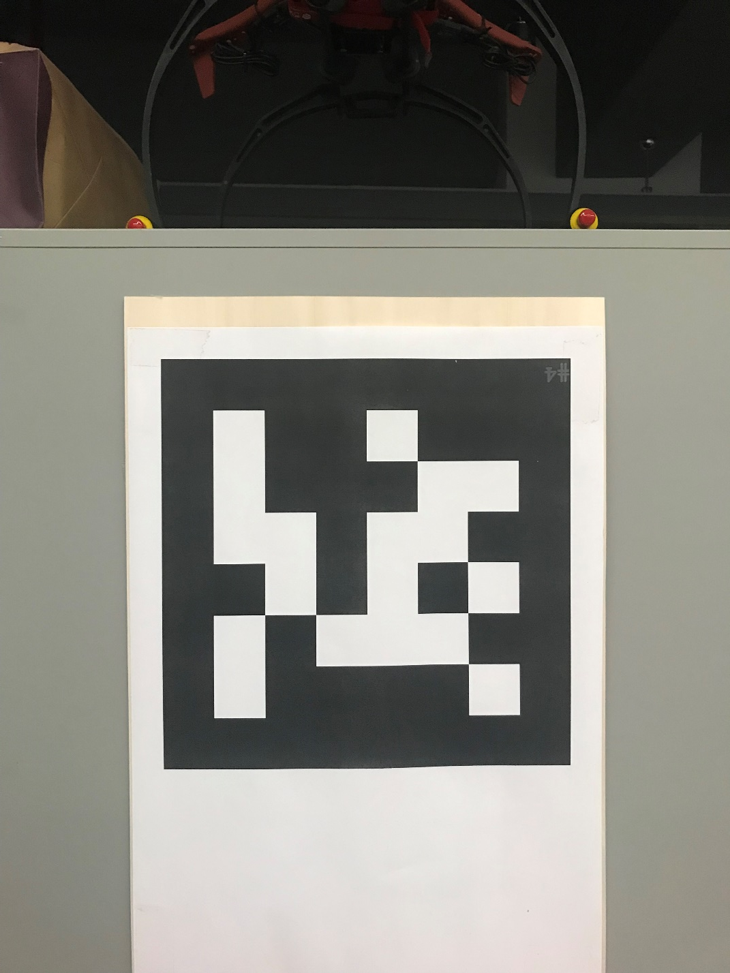
\includegraphics[height=6cm]{Aruco.png}}\hspace{4em}%
  \subcaptionbox{二维码原始图像\label{fig:Aruco_Gradient}}{%    
    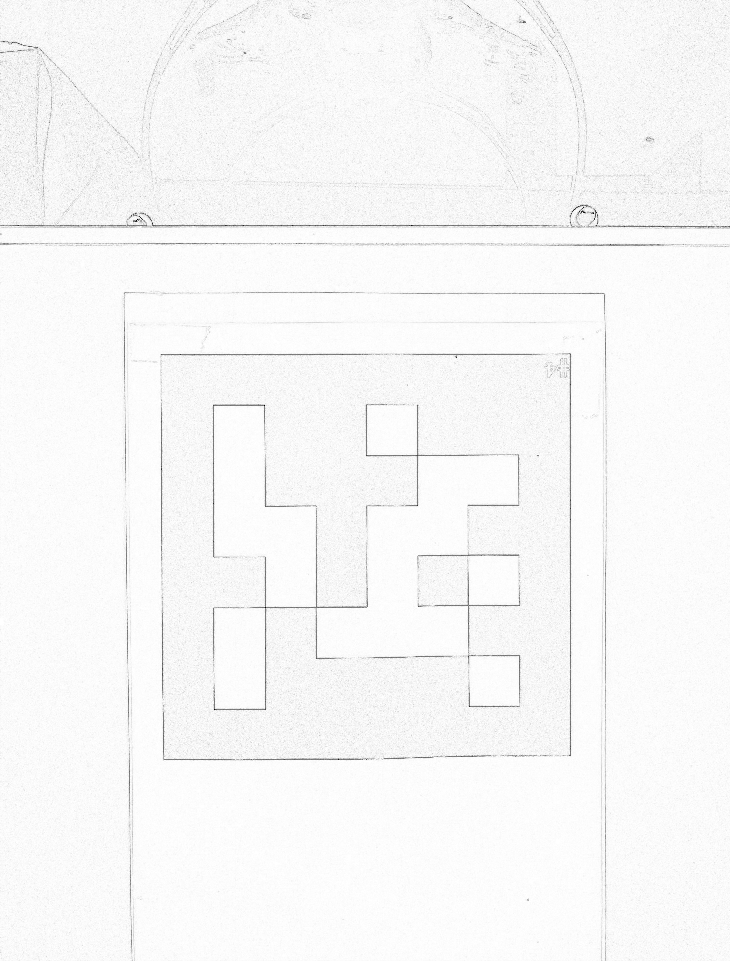
\includegraphics[height=6cm]{Aruco_Gradient.png}}
  \caption{二维码原始图像和梯度图}
  \label{fig:Aruco_Aruco_Gradient}
\end{figure}

ArUco的检测和识别过程主要包括检测出二维码4个角点在图像中的位置,以及被检出的二维码的ID序号,在检测4个角点的位置时,
需要检测图像中的线段和构成二维码的四边形。

在线段检测阶段,首先会计算整个图片中每一个像素的梯度强度大小和方向,随后对计算所得的梯度进行聚类,对所有满足聚类条
件的像素点进行合并,可以的得到一组连续点,即检测出线段。

检测完线段后,进一步的需要检测构成二维码边缘的四边形,针对上一步中获取到的所有线段,对线段进行分组,若满足,上一线
段的末端点和下一线段的起始点之间的距离小于某一阈值,即可首尾进行按照逆时针进行连接,若所有连接的线段数量达到4时,即
认定生成的闭环可能为一个二维码的边缘四边形。

在检测二维码ID值之前,会先设定好一个包含所有二维码的字典,字典的大小即二维码的数量,字典中元素的大小即是每一个二维
码的位数量。检测出构成二维码的四边形后,需要对图像进行透视变化规范图像,随后通过设定阈值分离出二维码上的黑色位和白
色位,通过位数情况即可判断该二维码是否是字典外的不合规值,以及字典中的特定ID值,识别结果如图~\ref{fig:Aruco_detection}
所示。通过这样的方式检测和识别二维码具备非常好的鲁棒性,并且可以对错误值进行效验。
\begin{figure}[H] % use float package if you want it here
  \centering
  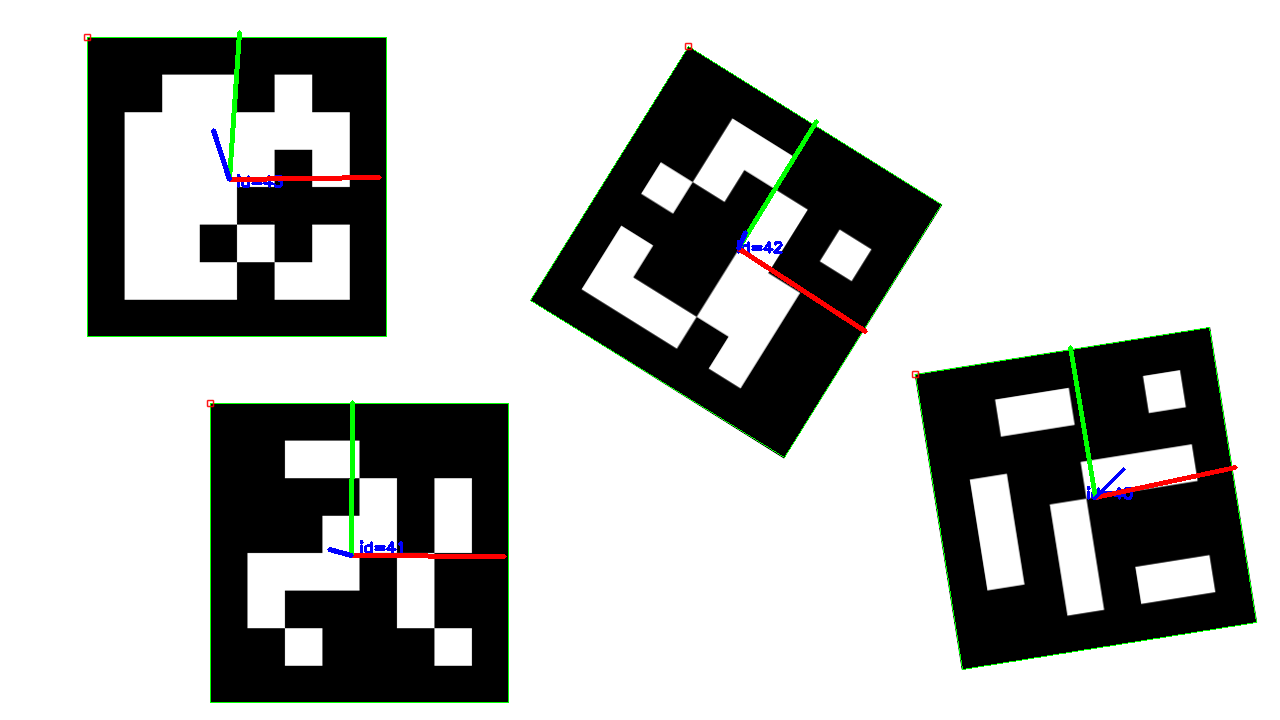
\includegraphics[height=6cm]{Aruco_detection.png}
  \caption{二维码识别结果示意图}
  \label{fig:Aruco_detection}
\end{figure}

\subsection{利用二维码估计相机外参}
\label{sec:2.2.3}
对于传入的单帧图像,在提取完二维码的四边形轮廓,4个角点以及检测对应的唯一ID值后,接下来会估计检出的二维码位姿,包括
平移向量和旋转向量,相机的外参主要是通过PnP方法,利用4对点来求解。

为了简化定位的过程,以二维码的坐标系作为世界坐标系,二维码边长为S,则四个角点的坐标分别为A(-S/2,S/2,0),
B(S/2,S/2,0),C(S/2,-S/2,0),D(-S/2,-S/2,0),在图像中的对应像素点为a($u_a$ ,$v_a$),
b($u_b$ ,$v_b$),c($u_c$ ,$v_c$),d($u_d$ ,$v_d$)。因为相机的内参K提前标定,则三维空间中的点和像素坐标中
的点之间的转换关系可以表示为:
\begin{equation}
\begin{split}
  Z{
  \left[ \begin{array}{ccc}
  a\\1
  \end{array} 
  \right ]}=Z{
  \left[ \begin{array}{ccc}
  u_a\\v_a\\1
  \end{array} \right ]}=K{
  \left[ \begin{array}{ccc}
  R&t
  \end{array} \right ]}{
  \left[ \begin{array}{ccc}
  A\\1
  \end{array} \right ]} \\
  ={
  \left[ \begin{array}{ccc}
  f_x & 0 & u_0\\0 & f_y &v_0 \\0 & 0 & 1
  \end{array} \right ]}{
  \left[ \begin{array}{cccc}
  r_{11}&r_{12}&r_{13}&t_1\\r_{21}&r_{7722}&r_{23}&t_2\\r_{31}&r_{32}&r_{33}&t_3
  \end{array} \right ]}{
  \left[ \begin{array}{ccc}
  -s/2\\s/2\\0\\1
  \end{array} \right ]}
\end{split}
\label{equ:mark2pose}
\end{equation}

通过公式~\ref{equ:mark2pose},可以通过二维码到的四个角点求解出相机的旋转矩阵和平移矩阵。
\section{联合二维码的SLAM系统描述}
\label{sec:2.3}
\subsection{引入二维码对SLAM优化研究}
\label{sec:2.3.1}
SLAM是一个在导航的过程中,进行建图的工作,在使用单目相机时,即使目前表现较好的ORB-SLAM或者LDSO等算法也很难达到预期想要的效果,
或者说存在很多的限制。第一个问题即是,所构成的地图的尺度是未知的,这样就造成无法在实际的导航任务中发挥作用,其次,在纯旋转的移
动过程中,会导致算法失效,第三个就是单目视觉SLAM往往需要场景中存在比较丰富的材质便于跟踪,最后还存在一个问题,当场景中的视点发
生变化,或者场景重复度较高时,在使用BOW词袋方法进行重定位时表现效果往往会很受到很大的限制。

除了用自然点来解决SLAM工作外,还有部分方法提出了仅仅使用人为设定的二维码来估计相机的位姿的方法,例如SPM-SLAM方法等,这种方式
就可以较好的解决上述问题。因为二维码的放置不需要按照特定的规则,可以按照实验人员根据具体场景来布置,这样做就可以的得到一个由二
维码构成的地图,并且,地图中的二维码都是具有尺度概念的。但是这样做存在的问题就是,我们需要在场景中布置足够多的二维码标志物,那
么在大尺度的场景中,这样做就会提高实验的难度,因为在相机移动的过程中,要时刻保证至少有两张二维码出现在本帧中。

基于上述两种情况,本文提出了一种融合自然特征点和人工放置的二维码的SLAM方法来解决各自的问题和限制。首先,对于实际实验环境中,能
够获取到真实的尺度概念,其次结合了自然点和二维码的SLAM方法也还可以可以只仅仅检测自然点,或者只检测二维码来进行位姿估计,因此对
于大多数场景,都可以有更好的鲁棒性,第三个优点在于每一个二维码都有一个单独准确得到的ID值,那么在高度重复的环境中,也能保证匹配
的正确性,最后对于大尺度的场景,可以结合自然点进行跟踪,二维码进行重定位来保证SLAM系统的长期稳定。

如图~\ref{fig:map}所示,对自然场景的局部区域进行建图,上图为自然区域的原图,在该区域中,有一部分的纹理较为丰富,其余部分则为贫纹理的白墙面,
在白墙面上人为布置二维码标志,下图为根据该区域重建出的3D地图,由图可见,在丰富纹理的区域,自然点和人为布置的二维码都可以检出,
但在贫纹理区域则,则基本只有二维码被检出,因此在贫纹理的区域就可以依靠二维码发挥作用。

\begin{figure}[htbp]
  \centering
    \subcaptionbox{自然场景}{\label{fig:cross}
    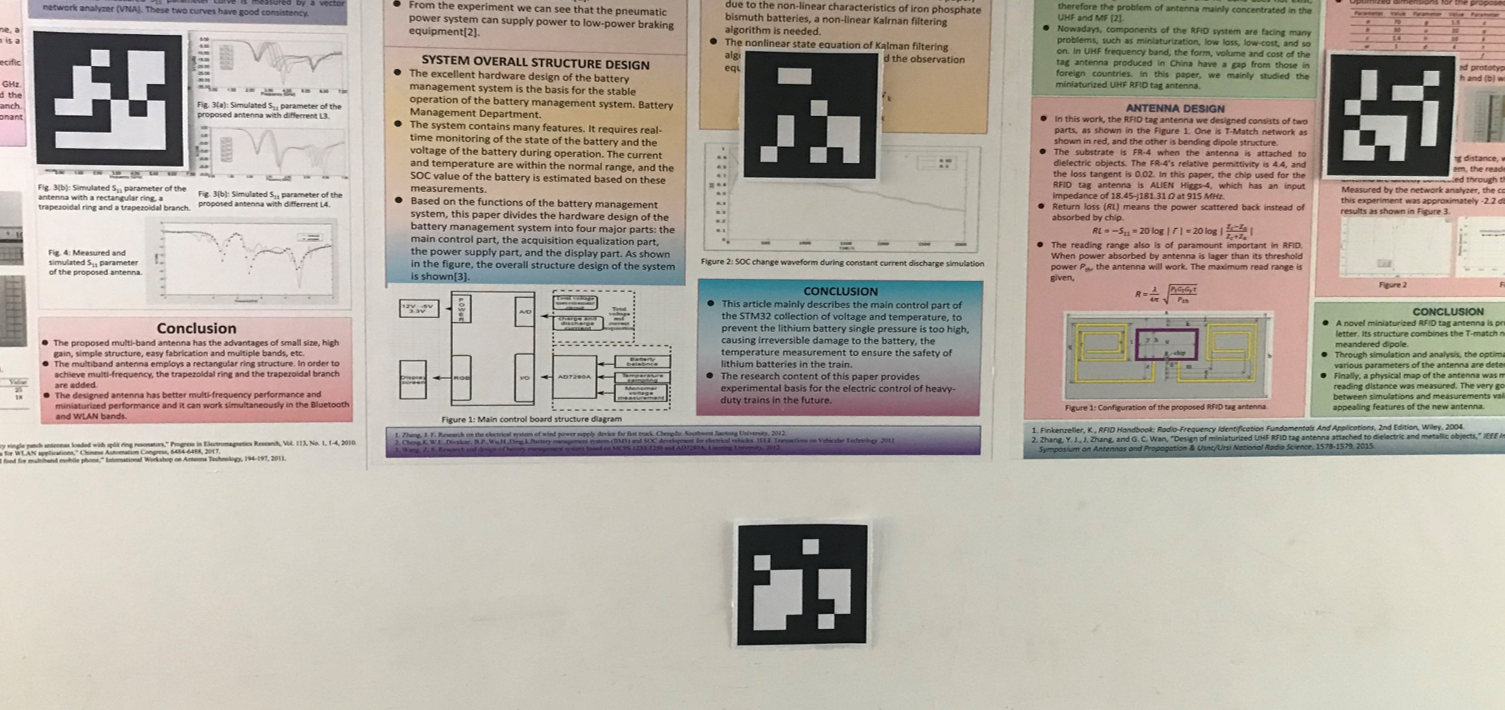
\includegraphics[width=12cm]{cross.png}\hskip2cm}
  \vskip0.5cm
    \subcaptionbox{根据自然场景建图}{\label{fig:cross_map}
    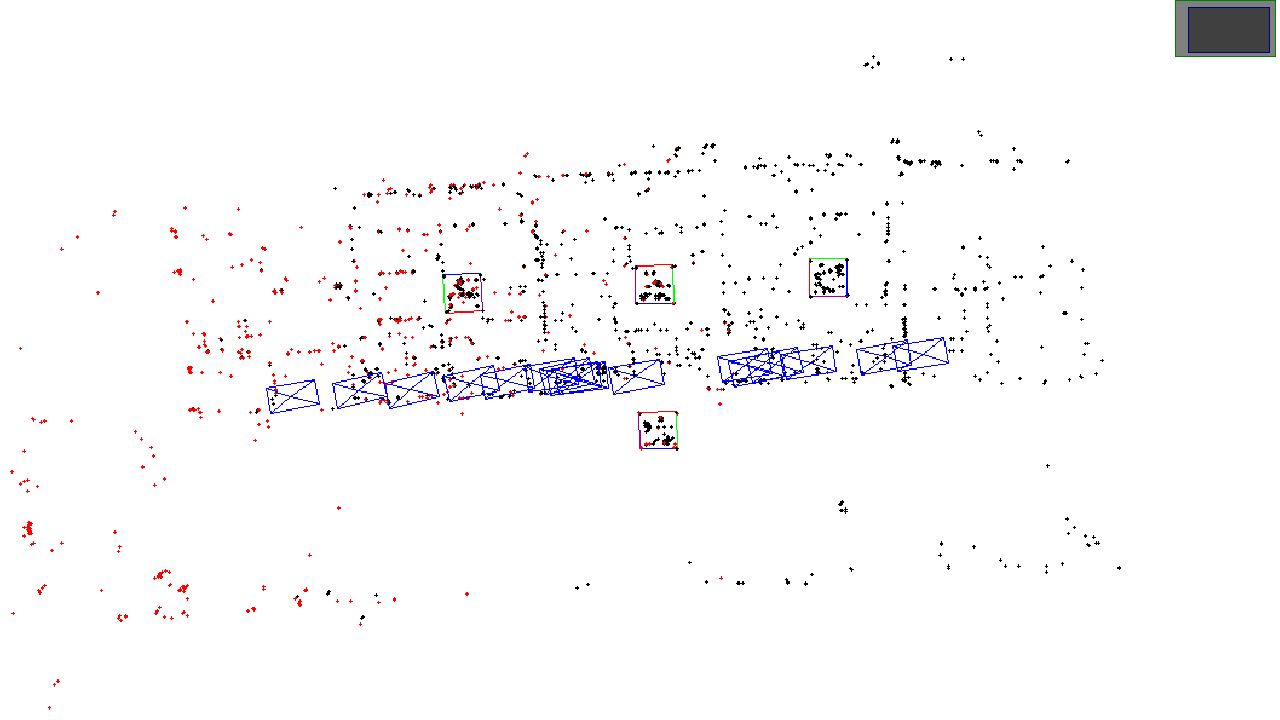
\includegraphics[width=12cm]{cross_map.png}\hskip2cm}
  \caption{包含二维码的构建地图示意图}\label{fig:map}
  \end{figure}

\subsection{包含二维码的地图描述}
\label{sec:2.3.2}
在SLAM运行的过程中,可以生成一套地图系统,对于同一场景,该系统能够复用于后续的建图和定位过程,通过这样得到的方式可以添加对系统
的约束,提高待估计量的精度。传统SLAM系统组成地图的元素主要包括关键点和关键帧,通过对关键点的描述符进行匹配,可以较好的的估计出
相机的位姿。但关键点描述符的计算和匹配过程一般都比较耗时,而且对于重复场景,非常用于出现匹配错误的情况,考虑到这一情况,本文在
此基础上,又添加二维码信息作为构成地图的元素,来进一步优化地图以获取更加准确得到相机位姿。

本文中地图的构成包括以下3个集合:关键点集合p,关键帧集合f和二维码m集合,每个集合之间的数据元素相互耦合关联。关键点集合
\begin{equation}p = \left\{x,v,d\right\}\end{equation}
其中每个元素代表三维空间中的一个点,该点的描述包括在地图坐标系中的三维坐标x,观测方向v以及该点的描述符信息d,考虑到SLAM系统的
实时性,选择BRIEF描述符来加快匹配过程。关键帧集合
\begin{equation}f = \left\{T,K\right\}\end{equation}
其中每一个关键帧包含一个外参矩阵矩阵T(旋转矩阵,平移矩阵),该外参矩阵是全局参考坐标系到相机参考坐标系的转化,K是相机的内参矩阵,
该参数包括相机焦距,光学中心以及畸变参数,这些参数需要在运行SLAM系统之前就准确测量得到。二维码集合
\begin{equation}m = \left\{s,M,x_1,x_2,x_3,x_4\right\}\end{equation}
其中的每一个二维码包括边长s(需要保证场景中的所有二维码的为正方形且所有二维码的尺度完全一致),二维码由其自身坐标系到全局坐标系的
转换矩阵M,$x_1$,$x_2$,$x_3$,$x_4$分别代表二维码四个角点在其自身坐标系下的坐标位置。通过对包含二维码的自然场景进行离线建图,所得地图
如图~\ref{fig:Ucoslam_map}所示,其中正方形代表检出的二维码,蓝色矩形代表检出关键帧,红色点代表检出关键点。
\begin{figure}[H] % use float package if you want it here
  \centering
  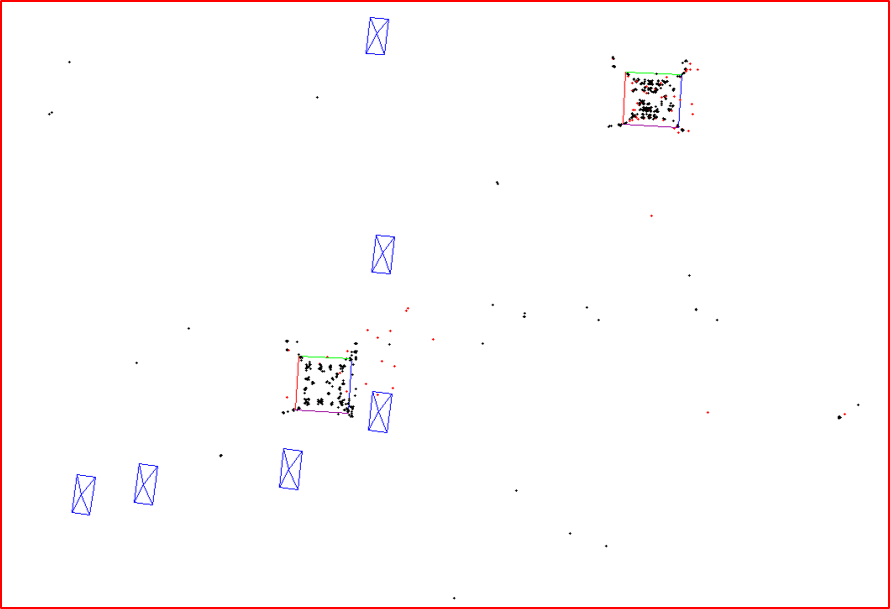
\includegraphics[height=6cm]{SLAM_Ucoslam_map.png}
  \caption{基于SLAM算法生成的地图}
  \label{fig:Ucoslam_map}
\end{figure}

其中每一类地图元素之间还具备一定的耦合关系,1)对于任意一个关键点,除了自身的属性外,还包括被观测帧序列,即所有可以观测到该特
征点的关键帧的集合,以及在这些帧中出现的像素坐标位置。2)对于任意一个关键帧,还包与其关联的其他关键帧序列,以及在该关键帧中所
有观测到的关键点和坐标。通过这些约束可以使得估计结果有更好的鲁棒性。

\subsection{联合二维码的SLAM过程描述}
\label{sec:2.3.3}
本文所提出的基于二维码的SLAM系统运行流程如图~\ref{fig:slam_pipeline}所示,与一般常见SLAM系统相比较,本文主要提出了结合关键点和二维码标记进行结合
使用。本方法中会一直对地图进行维护,有新的信息加入时,则会对地图进行不断的更新。在对某一个自然场景运行SLAM时,该地图为空,所
以需要对其进行初始化的工作。
\begin{figure}[H] % use float package if you want it here
  \centering
  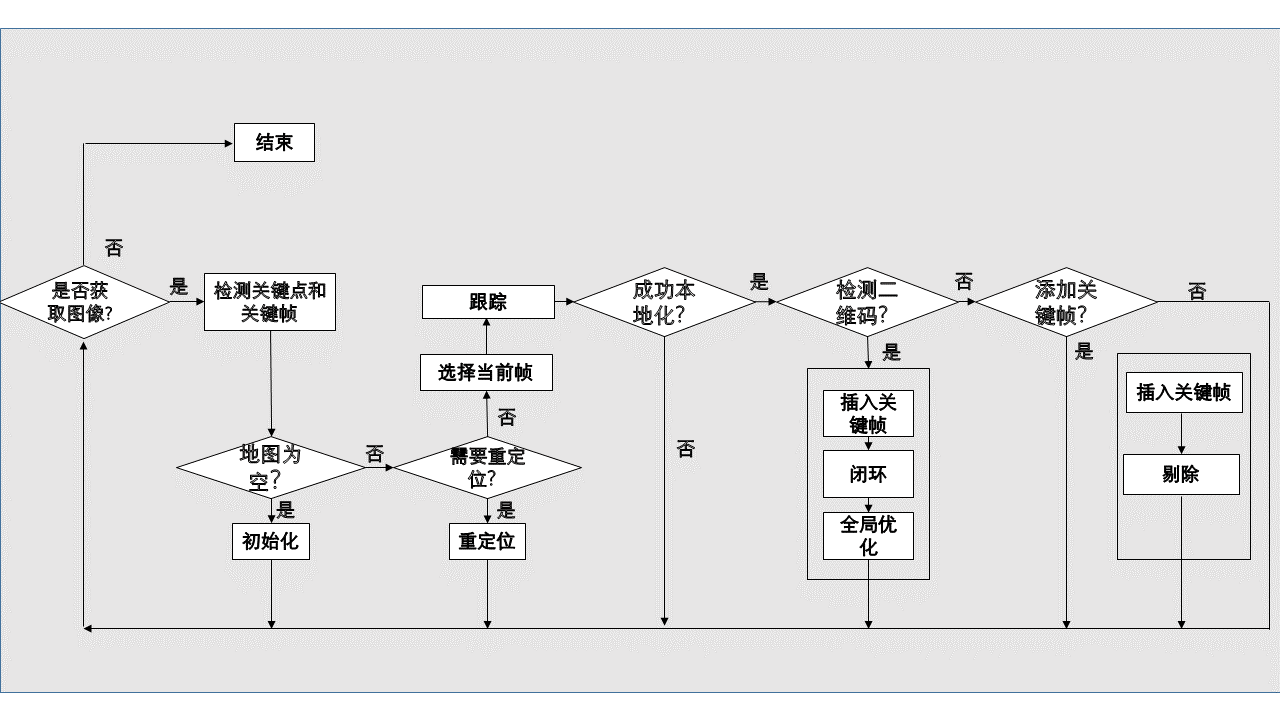
\includegraphics[height=9.5cm,width=14cm]{slam_pipeline.png}
  \caption{基于二维码的SLAM流程图}
  \label{fig:slam_pipeline}
\end{figure}
\textbf{地图初始化:}在SLAM中对地图的初始化可以获取相对尺度信息和参考坐标系的信息,主要是依靠多帧图像序列中关键帧或者二维码来完成,时
在一般情况下初始化的流程为:首先选择第一和第二帧($f_0$,$f_1$)运行两套初始化方法,如果任意一套方法初始化成功,那么就直接进入跟踪
环节;如果两套方案都初始化成功,则优先考虑使用二维码的初始化方式;如果都没有成功,那么则固定第一帧,换取第三帧重复上述过程
($f_2$,$f_3$...)。

对于基于关键点的初始化方法,它能够并行的计算初始帧之间的单应性矩阵和本质矩阵的鲁棒性方法,其中单应性矩阵一般用于场景为平面时,
其他场景则使用本质矩阵。在SLAM的过程里,只有检测到了足够大的视差时才会开始初始化,在单应矩阵和本质矩阵之间选择一个作为解算初
始化的矩阵,由于为了尽可能使得解具有足够的鲁棒性,导致由关键点进行初始化时很困难的。并且最重要的一点是,从关键点进行地图的初
始化,是无法获得尺度估计的,因此当在图像序列中一旦检测到二维码,系统就会对地图得到尺度进行调整以获得包含真实尺度的地图。

对于基于二维码的初始化方法,也是只要帧之间存在足足够的视差,就可以得到帧和二维码在地图中的位姿信息,但在某一帧中检测到多个二
维码标志时,则可以通过选择在该帧中最小化投影误差最小的二维码来解算初始化信息。使用二维码来进行初始化的一个优点就是,地图中的
参数都具备正确的尺度,因此就可以直接利用来为后续无人机的定位提供信息。

\textbf{跟踪模式:}如果在某一帧中估计出相机的位姿,则SLAM系统就会以前一帧作为起始点来估计当前帧的相机位姿,相机的位姿估计是将当前帧
中观测到的一组地图三维点和二维码角点进行重投影误差最小化得到过程,因此在该过程中主要包括两个步骤:寻找地图的对应关系和通过
最小化投影误差获取相机位姿。

在寻找地图点对应关系环节,首先,查找在前一帧中观察到的地图点与参考关键帧之间的匹配,因为他们很有可能再次出现在当前帧。通过这些
匹配可以解算出当前相机的初始估计;然后,通过将地图点投射到参考关键帧的相邻帧中来找到额外的匹配。对于每个地图点,首先需要检查
其视角与相机方向之间的夹角是否小于阈值,若大于则丢弃该点,然后,检查相机与地图点之间的欧氏距离是否在关键点的尺度不变性区域内
,随后,计算其投影,最后,将地图点的描述符与图像中搜索半径内的关键点进行比较。选择搜索半径中距离最小的两个关键点,且仅当描述
符之间的距离比大于0.8,以及最小的描述符距离低于最低阈值$\tau_d$, 则与匹配成功。一旦所有的匹配都被计算出来,重复的匹配就会被移除。
最终,关键点结合和检测到的二维码标记获得最终的精确位姿。

对于相机的位姿估计,以
\begin{equation}
\Upsilon_{p}^{f}=\{(\mathbf{p}, \mathbf{f}, \mathbf{g})\}
\end{equation}
和
\begin{equation}
\Upsilon_{p}^{\mathrm{f}}=\left\{\left(\mathbf{m}, \mathbf{f}, \mathbf{c}_{\mathbf{m}, \mathbf{f}}\right)\right\}
\end{equation}
表示通过上述步骤得到的$\mathrm{f}$帧中地图点和二维码标记的观测值,对于该帧的位姿$\mathbf{f}_{\mathrm{T}}$可以通过最小化重投影误差来估计:
\begin{equation}
\mathbf{f}_{\mathrm{T}}=\underset{\mathrm{T}}{\operatorname{argmin}}\left(\mathbf{w}_{\mathbf{p}}^{\mathrm{f}} H\left(\Upsilon_{p}^{\mathrm{f}}, \mathrm{T}\right)+\mathbf{w}_{\mathbf{m}}^{\mathrm{f}} H\left(\Upsilon_{m}^{\mathrm{f}}, \mathrm{T}\right)\right)
\label{equ:weight}
\end{equation}
其中
\begin{equation}
H\left(\Upsilon_{m}^{\mathrm{f}}, \mathrm{T}\right)=\sum_{\left(\mathrm{m}, \mathrm{f}, \mathrm{c}_{\mathrm{m}, \mathrm{f}}\right) \in \Upsilon_{m}^{\mathrm{f}}} \sum_{i=1}^{4}\left\|e\left(\mathrm{T} \cdot \mathbf{m}_{\mathrm{M}}, \mathbf{m}_{\mathrm{x}^{i}}, \mathbf{f}_{\delta}, \mathbf{c}_{\mathrm{m}, \mathrm{f}}^{i}\right)\right\|_{2}^{2}
\end{equation}
是当前帧观测到的二维码标记的重投影误差之和,其中
\begin{equation}
H\left(\Upsilon_{p}^{\mathrm{f}}, \mathrm{T}\right)=\sum_{(\mathbf{p}, \mathbf{f}, \mathbf{g}) \in \Upsilon_{p}^{\epsilon}} h_{\alpha}\left(e\left(\mathrm{T}, \mathbf{p}_{\mathbf{x}}, \mathbf{f}_{\delta}, \mathbf{g}_{u}\right) \Omega_{\mathbf{g}} e\left(\mathrm{T}, \mathbf{p}_{\mathbf{x}}, \mathbf{f}_{\delta}, \mathbf{g}_{u}\right)^{\top}\right)
\end{equation}
是当前帧观测到的地图点的重投影误差之和。对于Huber损失函数
\begin{equation}
h_{\alpha}(a)=\left\{\begin{array}{ll}{\frac{1}{2} a^{2}} & {\text { for }|a| \leq \alpha} \\ {\alpha\left(|a|-\frac{1}{2} \alpha\right)} & {\text { otherwise }}\end{array}\right.
\end{equation}
是为了降低优化过程中异常值的相对权重。

对于公式~\ref{equ:weight},二维码标记和地图点的权重分别由
$\mathbf{w}_{\mathbf{m}}^{\mathrm{f}}$
和$\mathbf{w}_{\mathbf{p}}^{\mathrm{f}}$决定,因为同以帧中地图点的数量远远多于二维码的个数,所以必须平衡两者之间的权重,
定义
\begin{equation}
\mathbf{w}_{\mathbf{p}}^{\mathbf{f}}=1-\mathbf{w}_{\mathbf{m}}^{\mathbf{f}}
\end{equation}
和
\begin{equation}
  \mathbf{w}_{\mathbf{m}}^{\mathbf{f}}=\frac{1}{2} \min \left(1, \frac{\mathbf{n}_{\mathbf{f}}}{\tau_{m}}\right)
\end{equation}
其中$\mathbf{n}_{\mathbf{f}}$代表追踪过程中该帧有效的二维码标记的个数,${\tau_{m}}$代表数量阈值,
$\mathbf{w}_{\mathbf{m}}^{\mathbf{f}}$的值将介于$\left[0, \frac{1}{2}\right]$之间,假设在追踪的过程中,没有检测到有效
的二维码,则$\mathbf{n}_{\mathbf{f}}$的值将为0,即该帧的位姿的结果将全部由地图点来估计。

\textbf{插入关键帧:}关键帧只有在向系统添加新信息时才会添加到地图中,以便实现平稳可靠的跟踪。因此,必须设定一些规则来确定是
否需要将当前帧添加至关键帧的集合。本文提出以下关键帧的提取规则:\\
1.如果当前帧至少有一个新的二维码标记出现(该标记没有出现在原本的地图中),则将该二维码和该帧添加到地图中。二维码是第一次在该帧
中被发现时添加的,因此也不能在帧中明确地估计该二维码的姿态。在这种情况下,标记的位姿被设置为无效,当观察标记的其他关键帧被添
加到地图中时,将对其进行估计。\\
2. 如果该帧包含至少一个二维码标记,且该二维码标记在地图中具有无效位姿,如规则1所描述,则该二维码的位姿可以在该帧中进行估计,
则添加该帧并更新该二维码在地图中的位姿。\\
3.如果帧包含至少一个二维码标志,并且距当前帧最近的关键帧的距离大于一个阈值$\tau_b$,该帧也会被添加进关键帧。\\
4 如果当前帧中匹配的映射点数量低于在参考关键帧中检测到的映射点总数的百分比$\tau_k$,该帧也会被添加进关键帧。

前三条规则的目的是考虑到当前关键帧中的可见二维码标记来检查是否添加关键帧,由于这些规则而没有被认为是关键帧的帧则通过最后一条
规则来添加。

本文中的SLAM系统再添加地图点是会遵循一种强鲁棒的策略,当一个新的关键帧被添加到地图时,系统有机会添加新的地图点,以及增加对现
有地图点的支持。对于每个关键点,搜索参考关键帧的相邻关键帧之间可能的对应,由于关键帧的姿态是已知的,所以采用了外极限制来减少
误检。一旦在地图上添加了一个点,将以一下侧率策略验证该点是否会被加入地图。基本思想是,该点必须至少在接下来的三分之二帧中可见,
直到再向地图添加两个关键帧。

\textbf{地图优化:}每次添加新的关键帧或检测到闭环时,都需要更新地图,以便加入新的信息,并剔除不正确的地图点。需要优化的元素
是关键帧位姿$k_T$、地图点位置$p_x$和二维码位姿$m_M$。

全局优化是一个缓慢耗时的过程,一次再SLAM中一般会议多线程的方式另外处理地图管理。然而,由于它是一个稀疏问题,因此可以使用稀疏
版本的Levenberg-Marquardt算法对其进行有效优化。只有在闭环结束之后才需要优化整个映射。当一个新的关键帧被添加到地图,只有地图
关键帧共享点需要更新,因此整个优化问题都属于局部优化。

\textbf{筛选关键帧:}与地图点的保存策略相似,关键帧剔除策略避免了关键帧的无限增长。但是,必须同时处理关键点和二维码标记。其
主要流程是,每个二维码标记和地图点应至少被三个关键帧所观测到,以便在进行优化过程时实现良好的三角化。对于每一个二维码标记m,
从关键帧集合中找到可以观测到的关键帧,并筛选出三个和该关键帧距离最近的关键帧,这些关键帧不会被筛除。对于剩余的关键帧,在不会
显著影响观察到的地图点的情况下会筛选掉,即某个关键帧中的地图点如果存在$\tau_c$的比例以上会被至少三个其他关键帧观测到,那
么该帧会被被认为是冗余的,而使用其他三个关键帧代替。

\textbf{回环检测和校准:}
在视觉SLAM中,对于相机位姿的解算都是由上一帧来计算的,那么这样就会造成误差的一直传递,产生累积误差,回环检测的提出就是通过建立
当前帧和历史帧之间的关系以减少累积误差。词袋模型的提出可以快速简单地完成回环检测,词袋模型使得每一帧都可以用单词来描述,表达为:
\begin{equation}
  F=1 \cdot \omega_{1}+0 \cdot \omega_{2}+0 \cdot \omega_{3}+\ldots+1 \cdot \omega_{n-1}+0 \cdot \omega_{n}
\end{equation}
每一帧$q$都可以由单词$w$和权重$\eta$构成:
\begin{equation}
  A=\left\{\left(w_{1}, \eta_{1}\right),\left(w_{2}, \eta_{2}\right), \ldots,\left(w_{N}, \eta_{N}\right)\right\} \triangleq v_{A}
\end{equation}
可以通过计算$q$,$d$两帧之间字典的相似度判断是否构成回环:
\begin{equation}
  \begin{aligned} s\left(v_{q}, v_{d}\right) &=1-\frac{1}{2}\left|\frac{v_{q}}{\left|v_{q}\right|}-\frac{v_{d}}{\left|v_{d}\right|}\right| \\ &=\frac{1}{2} \sum_{i | q_{i} \neq 0, d_{i} \neq 0}\left(\left|v_{q i}\right|+\left|v_{d i}\right|-\left|v_{q i}-v_{d i}\right|\right) \end{aligned}
\end{equation}
一旦相似度得到某一个阈值,就认为构成回环,检测到回环后,就可以通过历史帧来计算当前帧的位姿以减小误差。

在SLAM的运行过程中,当相机机在环境中移动时,不可避免地会产生漂移,必须对其进行检测和校正。在系统中,
回环检测必须区分关键点和二维码标记,使用关键点进行闭环检测时,一旦添加一个新的关键帧时,系统会另开辟一个线程进入地图管理模式,
因为SLAM系统会一直保留一个BoW数据库以检测是否插入关键帧,具体策略为: 测量最近添加的关键帧与图中相邻关键帧之间的相似性,保留
最低的$s_min$,然后对数据库进行查询,得到最相似的非邻居关键帧,相似度大于$s_min$。对于符合闭环的每个候选项,将使用插入的关
键帧计算其关键点对应关系。若对应数量足够大,则利用对应地图点的三维位置,利用RANSAC PnP方法,求出它们之间变换矩阵T 。如果转换
的内置点的数量足够高,则认为回环检测成功,随后进行校正。

另一方面,在处理任何其他帧之前,必须立即检测由二维码标记引起的闭环,如果在跟踪之前不纠正回环漂移,会导致相机的跟踪问题,因为
未纠正的帧位姿可能与二维码所计算出来的位姿差异较大。例如在某一个场景中,系统从一个二维码标记开始初始化,相机在场景中移动并回
到最初的起始位置,在这个过程中,会不断地叠加漂移误差,当相机第二次到达初始位置并再次观察二维码标记时,估计的相机姿态与实际会
较大,当使用二维码标记或关键点检测到循环闭合时,必须纠正漂移。

\textbf{重定位:}如果在跟踪的过程中失败们则必须进行重定位,重定位也是首先考虑使用二维码来完成,如果在某一帧中明确检测到二维
码标记,则利用该二维码来重新计算位姿,随后,通过查找地图对应关系和重新估计相机姿态来优化位姿。如果当前帧位姿不能从二维码标记
中准确地估计出来,就使用关键帧结合数据库进行查询,查询与当前帧相似的关键帧,并分析最佳关键帧。在回环检测出中,将当前帧的关键
帧与所选关键帧进行匹配,并采用RANSACPnP法估计相机的位姿T,如果内置点的数量足够高,则认为重新定位成功,系统重新进入跟踪模式。
\section{无人机定位系统设计}
\label{sec:2.4}
\subsection{无人机相机坐标变换数学描述}
\label{sec:2.4.1}
% 在SLAM系统中,常用的坐标系存在2个概念,分别是相机坐标系和世界坐标系。其中世界坐标系是我们最需要考虑的一个坐标系,世界坐标系代
% 表的是真实世界下,物体所参考的坐标系,一般都是固定不动的,可以给运动的物体提供控制方法,对于世界中的任意一点,可以描述
% 为P($X_w$,$Y_w$,$Z_w$)。相机坐标系代表的是移动的物体自身的坐标系,由于相机是刚性物体,一般以相机的坐标为准,对于相机中的任何一点,可
% 以描述为P($X_c$,$Y_c$,$Z_c$)。

% 因为SLAM系统中会涉及到多个坐标系,不同的坐标系之间需要进行转化,空间中点的坐标系变换是一个欧式变换,一般由旋转加平移构成。首先
% 只考虑坐标的纯旋转问题,即只有旋转,没有平移产生,两个坐标系的基底分别为($\vec {e_1}$,$\vec {e_2}$,$\vec {e_3}$)和
% ($\vec {e'_ 1}$,$\vec {e'_2}$,$\vec {e'_3}$)对应的坐标分别为($\vec {a_1}$,$\vec {a_2}$,$\vec {a_3}$)和($\vec {a'_1}$,$\vec {a'_2}$,$\vec {a'_3}$)。则有:
% \begin{equation}
% \begin{array}{l}\begin{bmatrix}\overrightarrow{e_1}&,\overrightarrow{e_2}&,\overrightarrow{e_3}\end{bmatrix}
% \begin{bmatrix}a_1\\a_2\\a_3\end{bmatrix}=\begin{bmatrix}\overrightarrow{e_1'}&,\overrightarrow{e_2'}&,\overrightarrow{e_3'}\end{bmatrix}
% \begin{bmatrix}a_1'\\a_2'\\a_3'\end{bmatrix}\\a\;=
% \begin{bmatrix}a_1\\a_2\\a_3\end{bmatrix}\;=
% \begin{bmatrix}e_1^Te_1'&e_1^Te_2'&e_1^Te_3'\\e_2^Te_1'&e_2^Te_2'&e_2^Te_3'\\e_3^Te_1'&e_3^Te_2'&e_3^Te_3'\end{bmatrix}
% \begin{bmatrix}a_1'\\a_2'\\a_3'\end{bmatrix}=Ra'\\\end{array}
% \end{equation}
% 其中旋转矩阵R由两组基之间的内积组成,表示坐标系旋转前后同一个向量的坐标变换关系。旋转矩阵是一个行列式为1的正交矩阵,满足以下特点:
% \begin{equation}RR^T=E(I),det(R)=I\end{equation}
% 则有:
% \begin{equation}a'=R^{-1}a=R^Ta\end{equation}
% 在欧式变换中,除了旋转还有平移:
% \begin{equation}a'=Ra+t\end{equation}
% 可以用旋转矩阵R和平移向量t就能描述空间中的坐标变换关系
% \begin{equation}
% \begin{bmatrix}a'\\1\end{bmatrix}=
% \begin{bmatrix}R&t\\0^T&1\end{bmatrix}
% \begin{bmatrix}a\\1\end{bmatrix}=T
% \begin{bmatrix}a\\1\end{bmatrix}
% \end{equation}
% 在三维向量的末尾添加1,称为齐次坐标。矩阵T同时包含了旋转和平移,称为变换矩阵。

无人机上携带的相机可以看成三维空间中的刚体(保证了同一个向量在各个坐标系下的长度和夹角都不会发生变化)因此需要考虑相机的位姿,即旋转和平移。
对于平移可以利用向量来表示,旋转则利用旋转矩阵,旋转向量,欧拉角,四元数等方式来描述,本文也将主要说明旋转过程的数学描述。

\textbf{旋转矩阵:}对于任意向量{~p~},在两个坐标系的描述为:
\begin{equation}
  \left[\mathbf{e}_{1}, \mathbf{e}_{2}, \mathbf{e}_{3}\right]\left[\begin{array}{l}{a_{1}} \\ {a_{2}} \\ {a_{3}}\end{array}\right]=\left[\mathbf{e}_{1}^{\prime}, \mathbf{e}_{2}^{\prime}, \mathbf{e}_{3}^{\prime}\right]\left[\begin{array}{c}{a_{1}^{\prime}} \\ {a_{2}^{\prime}} \\ {a_{3}^{\prime}}\end{array}\right]
\end{equation}

等式两边同时左乘$\left[\begin{array}{ccc}{\mathbf{e}_{1}^{T},} & {\mathbf{e}_{2}^{T},} & {\mathbf{e}_{3}^{T}}\end{array}\right]^{T}$可得
\begin{equation}
\left[\begin{array}{l}{a_{1}} \\ {a_{2}} \\ {a_{3}}\end{array}\right]=\left[\begin{array}{lll}{e_{1}^{T} e_{1}^{\prime}} & {e_{1}^{T} e_{2}^{\prime}} & {e_{1}^{T} e_{3}^{\prime}} \\ {e_{2}^{T} e_{1}^{\prime}} & {e_{2}^{T} e_{2}^{\prime}} & {e_{2}^{T} e_{3}^{\prime}} \\ {e_{3}^{T} e_{1}^{\prime}} & {e_{3}^{T} e_{2}^{\prime}} & {e_{3}^{T} e_{3}^{\prime}}\end{array}\right]\left[\begin{array}{c}{a_{1}^{\prime}} \\ {a_{2}^{\prime}} \\ {a_{3} ;}\end{array}\right]=\mathbf{R a}^{\prime}
\end{equation}

对于旋转矩阵R,即可描述旋转过程,并且R可以定义为特殊正交群:
\begin{equation}
  S O(n)=\left\{\mathbf{R} \in R^{n \times n} | \mathbf{R} \mathbf{R}^{T}=\mathbf{I}, \operatorname{det}(\mathbf{R})=1\right\}
\end{equation}

\textbf{旋转向量:}旋转矩阵在描述旋转时存在参数冗余和自身约束的问题,因此提出一个更加紧凑的数学描述$\theta_{n}$,旋转向量方向为旋转轴{~n~},
大小为旋转角$\theta$。旋转向量和旋转矩阵的转换可以用罗德里格斯公式表示:
\begin{equation}
  \mathbf{R}=\cos \theta \mathbf{I}+(1-\cos \theta) \mathbf{n} \mathbf{n}^{T}+\sin \theta \mathbf{n}^{\wedge}
\end{equation}

反之则有
\begin{equation}
  \operatorname{tr}(\mathbf{R})=\cos \theta \operatorname{tr}(\mathbf{I})+(1-\cos \theta) \operatorname{tr}\left(\mathbf{n} \mathbf{n}^{T}\right)+\sin \theta \operatorname{tr}\left(\mathbf{n}^{\wedge}\right)=1+2 \cos \theta
\end{equation}

\textbf{欧拉角:}将旋转运动分解成分别绕三个坐标轴的旋转($[r, p, y]^{T}$)来表示的,三个旋转的总和即为总的旋转,表述最为直观。

\textbf{四元数:}由于欧拉角和旋转向量存在奇异性,且不存在不带奇异性的三维向量描述方式,因此提出四元数这种紧凑且没有奇异性的数学
描述。四元数可以描述为:
\begin{equation}
  \mathbf{q}=q_{0}+q_{1} i+q_{2} j+q_{3} k=\{s, \mathbf{v}\}
\end{equation}
可以用单位四元数来描述空间中的任意旋转,假设旋转的描述为$\theta_{n}$,则:
\begin{equation}
  \mathbf{q}=\left[\cos \frac{\theta}{2}, n_{x} \sin \frac{\theta}{2}, n_{y} \sin \frac{\theta}{2}, n_{z} \sin \frac{\theta}{2}\right]^{T}
\end{equation}
旋转描述为R时,则:
\begin{equation}
\mathbf{R}=\left[\begin{array}{ccc}{1-2 q_{2}^{2}-2 q_{3}^{2}} & {2 q_{1} q_{2}-2 q_{0} q_{3}} & {2 q_{1} q_{3}+2 q_{0} q_{2}} \\ {2 q_{1} q_{2}+2 q_{0} q_{3}} & {1-2 q_{1}^{2}-2 q_{3}^{2}} & {2 q_{2} q_{3}-2 q_{0} q_{1}} \\ {2 q_{1} q_{3}-2 q_{0} q_{2}} & {2 q_{2} q_{3}+2 q_{0} q_{1}} & {1-2 q_{1}^{2}-2 q_{2}^{2}}\end{array}\right]
\end{equation}
反之则有:
\begin{equation}
  q_{0}=\frac{\sqrt{\operatorname{tr}(\mathbf{R})+1}}{2}, q_{1}=\frac{m_{23}-m_{32}}{4 q_{0}}, q_{2}=\frac{m_{31}-m_{13}}{4 q_{0}}, q 3=\frac{m_{12}-m_{21}}{4 q_{0}}
\end{equation}
通过以上方式都可以描述刚性运动中的旋转过程R,结合物体的平移t,则变化后的坐标为:
\begin{equation}
  \mathbf{a}^{\prime}=\mathbf{R} \mathbf{a}+\mathbf{t}
\end{equation}

在实际的使用中,由于以上等式非线性,可以引入齐次坐标T,可以将上式改成:
\begin{equation}
\left[\begin{array}{l}{\mathbf{a}^{\prime}} \\ {1}\end{array}\right]=\left[\begin{array}{ll}{\mathbf{R}} & {\mathbf{t}} \\ {\mathbf{0}^{T}} & {1}\end{array}\right]\left[\begin{array}{l}{\mathbf{a}^{\prime}} \\ {1}\end{array}\right]=\mathbf{T}\left[\begin{array}{l}{\mathbf{a}} \\ {1}\end{array}\right]
\end{equation}

对于变换矩阵T,可以定义为特殊欧氏群:
\begin{equation}
S E(3)=\left\{T=\left[\begin{array}{cc}{\mathbf{R}} & {\mathbf{t}} \\ {\mathbf{0}^{T}} & {1}\end{array}\right] \in R^{4 \times 4} | \mathbf{R} \in S O(3), t \in R^{3}\right\}
\end{equation}

对于针孔相机模型,如图~\ref{fig:2VSLAM_pinehole}所示,(其中f为相机焦距)存在4个坐标系分别为:世界坐标系,相机坐标系,图像坐
标系和像素坐标系,对于真实世界中的空间点$P_w$($X_w$,$Y_w$,$Z_w$),其对应的相机坐标系坐标为$P_c$($C_w$,$C_w$,$C_w$),
对应的图像坐标系为$P^{'}$($X^{'}$,$Y^{'}$),对应的像素坐标系为p(u,v)。
\begin{figure}[H] % use float package if you want it here
  \centering
  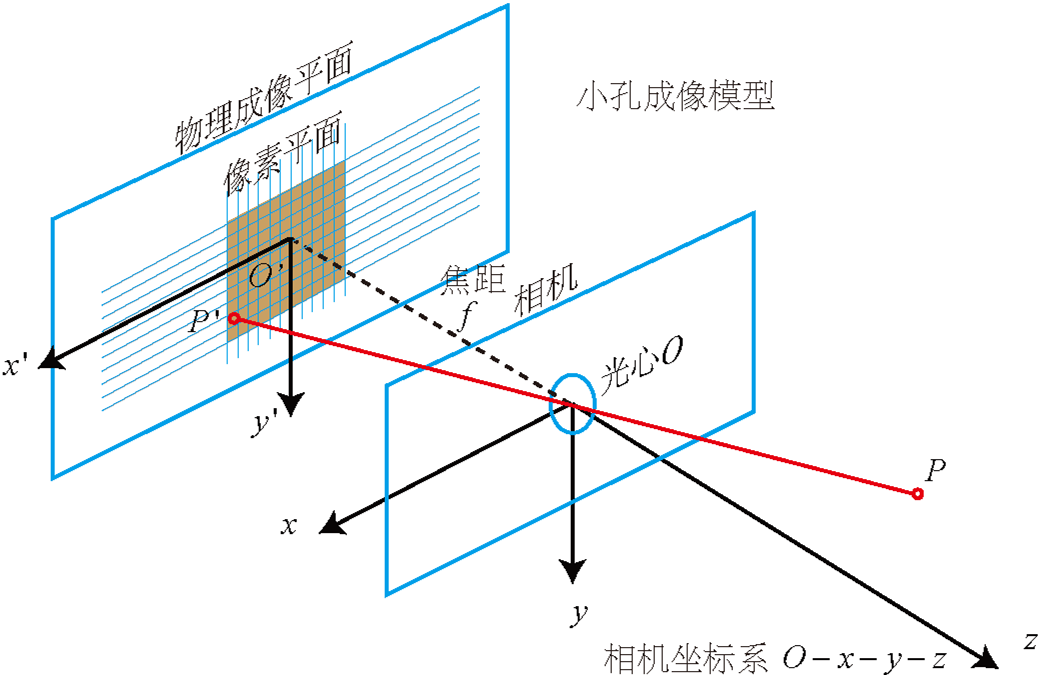
\includegraphics[height=6cm]{2VSLAM_pinehole.png}
  \caption{针孔相机模型}
  \label{fig:2VSLAM_pinehole}
\end{figure}
对于世界坐标系到相机坐标系之间的转化:
\begin{equation}
  \left[\begin{array}{l}{X c} \\ {Y_{C}} \\ {Z_{C}}\end{array}\right]=R\left[\begin{array}{l}{X w} \\ {Y w} \\ {Z w}\end{array}\right]+t
  \label{equ:world2cam}
\end{equation}
对于相机坐标系到图像坐标系之间的转化,可以利用如图~\ref{fig:2VSLAM_similartri}所示的相似三角形来求解:
\begin{equation}
  \begin{split}
    \frac{Z c}{f}=\frac{X c}{X^{'}}=\frac{Y c}{Y^{'}}\\
    \left\{\begin{array}{l}{X^{\prime}=f \frac{X c}{Z c}} \\ {Y^{\prime}=f \frac{Y c}{Z c}}\end{array}\right.
\end{split}
\label{equ:cam2photo}
\end{equation}
对于图像坐标系到像素坐标系的转化,如图~\ref{fig:2VSLAM_pixeltrans}所示:
\begin{equation}
  \begin{split}
    \left\{\begin{array}{l}{u=\frac{X^{\prime}}{d_{x}}+u_{o}} \\ {v=\frac{Y^{\prime}}{d_{y}}+v_{o}}\end{array}\right.\\
    \left[\begin{array}{l}{u} \\ {v} \\ {1}\end{array}\right]=\left[\begin{array}{ccc}{\frac{1}{d_{x}}} & {0} & {u_{o}} \\ {0} & {\frac{1}{d_{x}}} & {v_{o}} \\ {0} & {0} & {1}\end{array}\right]\left[\begin{array}{c}{X^{\prime}} \\ {Y^{\prime}} \\ {1}\end{array}\right]
  \end{split}
  \label{equ:photo2pixel}
\end{equation}
\begin{figure}[H]
  \centering%
  \subcaptionbox{相机坐标系到图像坐标系转换\label{fig:2VSLAM_similartri}}{%    
    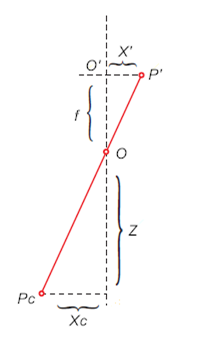
\includegraphics[height=4cm]{2VSLAM_similartri.png}}\hspace{6em}%
  \subcaptionbox{图像坐标系到像素坐标系转换\label{fig:2VSLAM_pixeltrans}}{%    
    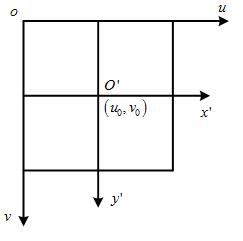
\includegraphics[height=4cm]{2VSLAM_pixeltrans.png}}
  \caption{坐标系转化示意图}
  \label{fig:trans}
\end{figure}
其中$d_x$,$d_y$分别表示沿着x,y轴的实际物理尺寸,($u_o$,$v_o$)表示光心对应到像素坐标系得到坐标.由公式~\ref{equ:cam2photo}和
~\ref{equ:photo2pixel}可以转化得到相机坐标系到像素坐标系的关系:
\begin{equation}
Z c\left[\begin{array}{l}{u} \\ {v} \\ {1}\end{array}\right]=\left[\begin{array}{ccc}{\frac{f}{d_{x}}} & {0} & {u_{0}} \\ {0} & {\frac{f}{d_{y}}} & {v_{0}} \\ {0} & {0} & {1}\end{array}\right]\left[\begin{array}{c}{X_{c}} \\ {Y_{c}} \\ {Z_{c}}\end{array}\right]=\left[\begin{array}{ccc}{f_{x}} & {0} & {u_{0}} \\ {0} & {f_{y}} & {v_{0}} \\ {0} & {0} & {1}\end{array}\right]\left[\begin{array}{c}{X_{c}} \\ {Y_{c}} \\ {Z_{c}}\end{array}\right]=K\left[\begin{array}{c}{X_{c}} \\ {Y_{c}} \\ {Z_{c}}\end{array}\right]
  \label{equ:cam2pixel}
\end{equation}
由公式~\ref{equ:world2cam}和~\ref{equ:cam2pixel}得到世界坐标系到像素坐标系的转化关系为:
\begin{equation}
Z c\left[\begin{array}{l}{u} \\ {v} \\ {1}\end{array}\right]=K(R P w+t)=K\left(R\left[\begin{array}{l}{X w} \\ {Y w} \\ {Z w}\end{array}\right]+t\right)
\end{equation}
其中K表示相机内参矩阵,R,t表示相机外参。
\subsection{获取真实世界坐标系方法}
\label{sec:2.4.2}
在SLAM系统中所描述的定位信息都是基于地图坐标系或者相机坐标系,但是在实际的应用中,就需要将所有的定位信息全部转换至真实世界坐标系,
才能为物体后续的移动提供控制方法。我们通过传统的SLAM方法,只能够得相机在地图坐标系中的位姿,现得益于二维码自带坐标系的特性,可以
经过一定的转换可以获取相机在真实世界坐标系下的位姿,可以为后续控制提供真实的位姿信息。

首先,声明所有可以得到的坐标信息,可以通过SLAM系统得到,二维码在SLAM地图坐标系下的位姿$T_{marker}^{c}$,
相机在SLAM地图坐标系下得到位姿$T_{camera}^{c}$,二维码在真实世界坐标系的位姿$T_{marker}^{w}$。
经过坐标变化,可以的得到相机在二维码下的位姿
\begin{equation}
T_{camera}^{m} =\begin{bmatrix}T_{marker}^{c}\end{bmatrix}^{-1}T_{camera}^{c}
\end{equation}
真实世界坐标系在二维码坐标系下的位姿
\begin{equation}
T_{world}^{m} =\begin{bmatrix}T_{marker}^{w}\end{bmatrix}^{-1}
\end{equation}
那么相机在真实世界坐标系下的位姿
\begin{equation}
\begin{array}{l}T_{camera}^w=
\begin{bmatrix}T_{world}^m\end{bmatrix}^{-1}T_{camera}^m\\=\;T_{marker}^w
\begin{bmatrix}T_{marker}^c\end{bmatrix}^{-1}T_{camera}^c\end{array}
\end{equation}

其中,二维码在真实世界坐标系的位姿可以按照实际场景进行设置,为了计算方便,直接设定第一个二维码的中心点为世界坐标系三维坐标的
中心点,且x轴朝右,y轴朝上,z轴垂直于二维码平面向外,如图~\ref{fig:Aruco_global}所示,那么第一个二维码的在世界坐标系下的坐
标为(0,0,0),其余二维码则可以按照真实尺度获取。
\begin{figure}[H] % use float package if you want it here
  \centering
  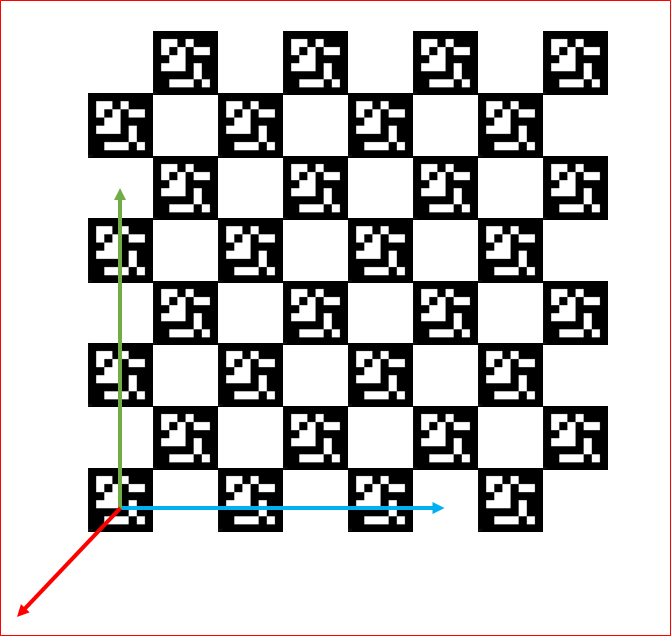
\includegraphics[height=6cm]{Aruco_global.png}
  \caption{二维码布置示意图}
  \label{fig:Aruco_global}
\end{figure}
在SLAM的实际运行前,应该保证二维码的实际布置坐标和设定的二维码在实际世界坐标系下的坐标一致,避免SLAM过程中位姿的抖动问题,先
验地图可以设定以配置文件的形式记录,这样可以针对不同的场景和不同的二维码布置情况,直接修改配置文件即可。
在SLAM的运行过程中,应该尽可能保证每一帧都可以看到至少一个二维码,,对于观测不到二维码的图像帧,SLAM算法将利用特征点匹配进行
定位,当观测的图像帧中有多个二维码时,那么就需要考虑到多个二维码的协同影响,处理方式有如下几种形式:\\
1 提前选择某一个参考二维码,无论相机观测到哪一个二维码,都根据观测到的二维码和参考二维码之间的位姿关系,求解相机在世界坐标系
下的位姿。\\
2.对于观测到的多个二维码标记,根据上一帧计算出来的位姿,可以计算出当前帧距离最近的一个二维码,以该二维码作为参考,计算出此时
相机在世界坐标系下的位姿。\\
3. 对于观测到的多个二维码标记,分别结合各个二维码计算出此时相机在世界坐标系下的位姿,对于所有位姿,求取平均值即可。

以上三种方法都可以解算出相机在真实世界坐标系下的位姿,其中方法1的计算过程最为简略,并且全程只利用一个参考二维码可以避免在
频繁更换参考二维码的过程中造成的位姿抖动问题,但是会存在线性放大相机位姿误差的情况,该方法难以对误差进行优化。方法2会应用
到历史位姿信息,可以有效降低相机误差,当时会频繁更换参考二维码,这样也会造成相机位姿估计过程的抖动问题。方法3.和方法2类
似,在处理误差时会结合多个参考二维码的信息,使得估计位姿的系统鲁棒性提升。针对不同的场景,需要结合具体的方法,对于二维码远
距离线性摆放的场景,应该避免使用方法1,优先考虑方法2和方法3;对于实时性要求较高的场景,则优先考虑方法1。


% \begin{algorithm}[!h]
  % 	\caption{PARTITION$(A,p,r)$}%算法标题
  % 	\begin{algorithmic}[1]%一行一个标行号
  % 		\STATE $i=p$
  % 		\FOR{$j=p$ to $r$}
  % 		\IF{$A[j]<=0$}
  % 		\STATE $swap(A[i],A[j])$
  % 		\STATE $i=i+1$
  % 		\ENDIF
  % 		\ENDFOR
  % 	\end{algorithmic}
  % \end{algorithm}
\subsection{无人机自主定位设计}
\label{sec:2.4.3}
根据以上章节,可以确定出在真实世界下相机的位姿结果,在具体的工程实践中,除了结合二维码的SLAM算法的研究,还需要考虑到先验地图
的设定,数据的传输,相机的设定等问题,具体流程如图\ref{fig:getPose_pipeline}所示。
\begin{figure}[t] % use float package if you want it here
  \centering
  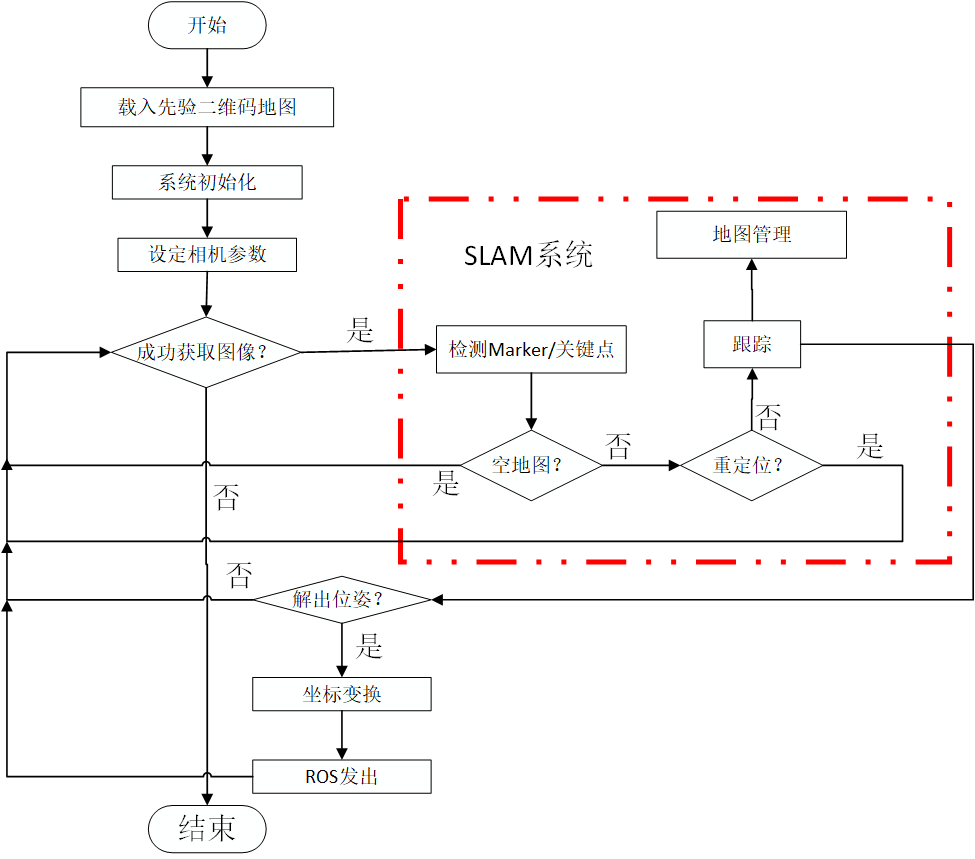
\includegraphics[height=14cm]{getPose_pipeline_1.png}
  \caption{获取真实位姿完整流程图}
  \label{fig:getPose_pipeline}
\end{figure}


\textbf{地图管理:}地图设定:在无人估计位姿时,如果有先验地图的加入,则可以添加约束进一步优化位姿结果。在载入地图的过程中,
如果该场景是第一次测量,没有先验的地图信息,则创建一个空的globalmap来存储地图信息,并将MapFlag字段设定为NotFirstMap;
反之,则直接载入历史先验地图。在整个定位流程结束后,将更新后的地图保存在globalmap中。
\begin{lstlisting}[
  language=C++,
  numbers=left,                
  numberstyle=\footnotesize,
  frame=single,     
  basicstyle=\small\tt,    
  escapeinside = '',
  caption={地图管理~C++~实现},
  label={code:loadMarkermap}]
'//载入地图'
if (Map_Flag == NotFirst_Map) 
	{
    globalmap->readFromFile(map_path);
  }
else
	{
    globalmap->readFromFile(map_path);
	  Map_Flag == NotFirst_Map;
	}
'//保存地图'
if (Map_Flag == Save_Map) 
    {globalmap->saveToFile(map_path);}
\end{lstlisting}

\textbf{载入先验二维码地图:}载入先验二维码地图:首先准备先验地图配置文件,包括二维码的真实尺度,所有二维码的ID值,以及每一
个二维码特定的id值和在真实世界坐标系下的位姿(R,t)。如代码~\ref{code:loadMarkermap}所示,需要依次遍历每个二维码的信息,
最终将所有数据都存储在markermap中。
\begin{lstlisting}[
  language=C++,
  numbers=left,                
  numberstyle=\footnotesize,
  frame=single,     
  basicstyle=\small\tt,    
  escapeinside = '',
  caption={载入先验二维码地图~C++~实现},
  label={code:loadMarkermap}]

'先验地图配置文件:'
  %YAML:1.0
  markersize: 0.73
  markers_id: [0,1]
  id_0: !!opencv-matrix
  rows: 4
  cols: 4
  dt: d
  data: [1.0, 0.0, 0.0, 0.0, 
        0.0, 1.0, 0.0, 0.0,  
        0.0, 0.0, 1.0, 0.0, 
        0.0, 0.0, 0.0, 1.0]
  id_1: !!opencv-matrix
  rows: 4
  cols: 4
  dt: d
  data: [1.0, 0.0, 0.0, 4.0, 
          0.0, 1.0, 0.0, 0.0,  
          0.0, 0.0, 1.0, 0.0, 
          0.0, 0.0, 0.0, 1.0]

'先验地图载入代码:'
  void loadMarkermap(string path){
    cv::FileStorage fs(path, cv::FileStorage::READ);
    fs["markersize"] >> markersize;
    fs["markers_id"] >> markers_id;
    for (std::size_t  i =0;i<markers_id.size();i++){
        cv::Mat cvmarker ;
        Eigen::Matrix<double,4,4> marker;
        fs["id_"+to_string(markers_id[i])] >> cvmarker;
        cv2eigen(cvmarker,marker);
        markermap[markers_id[i]] = marker;
    }
  }
\end{lstlisting}

\textbf{设定SLAM参数:}对于结合二维码的SLAM系统,需要对系统中的参数进行设定,主要包括SLAM的运行模式(SLAM模式,重定位模式)
,特征点的提取方式(orb、brief、SIFT等),二维码的检测类别(ARUCO\_MIP\_25h7、ARUCO\_MIP\_36h12等),关键帧筛选阈值,线程的数
量,是否复用地图等等,这些SLAM相关的参数都需要在运行前设定,具体内容如代码~\ref{code:setSlam}所示。

\begin{lstlisting}[
  language=C++,
  numbers=left,                
  numberstyle=\footnotesize,
  frame=single,     
  basicstyle=\small\tt,    
  escapeinside = '',
  caption={slam启动和参数设置~C++~实现},
  label={code:setSlam}]
  void setSlam(int argc){
      UcoSlamParams.runSequential=false;
      UcoSlamParams.detectMarkers=true;
      UcoSlamParams.aruco_markerSize=markersize;
      UcoSlamParams.aruco_Dictionary="ARUCO_MIP_36h12";
      UcoSlamParams.nthreads_feature_detector =1;
  }
\end{lstlisting}
\textbf{设定相机参数:}相机的选择对基于纯视觉的无人机定位任务也很重要,作为SLAM系统的输入,必须选择一台成像质量高,稳定性强的相机。在实际工程中选择PointGrey 
(CM3-U3-31S4M-CS)工业相机来接受视觉信息,外形如图~\ref{fig:getPose_pt}所示,具体参数如表~\ref{tab:pointgrey}所示。

相机在使用过程中需要设定的参数一般包括相机内参,以及曝光,快门时间和增益等,对于相机内参需要提前进行标定,后面三个参数需要根据实际场景调试后确定出最佳数值。
\begin{figure}[H] % use float package if you want it here
  \centering
  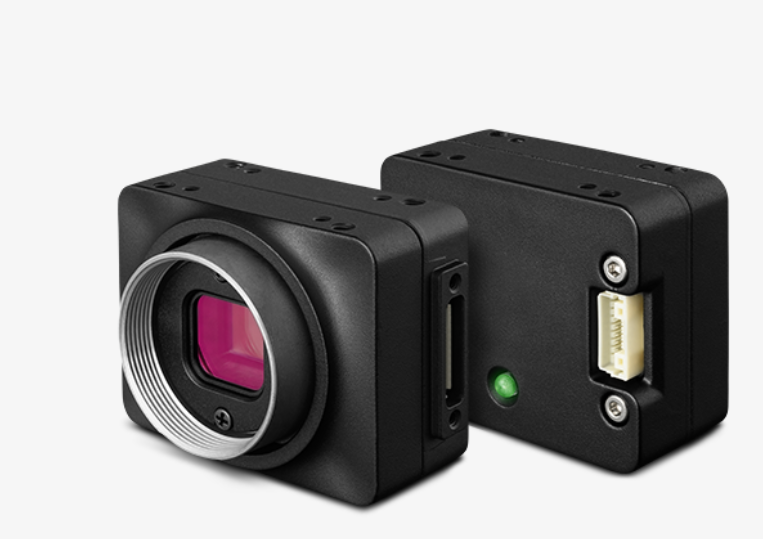
\includegraphics[height=6cm]{getPose_pt.png}
  \caption{PointGrey工业相机示意图}
  \label{fig:getPose_pt}
\end{figure}

\begin{table}[h]
  \centering
  \caption{pointgrey相机参数表}
  \label{tab:pointgrey}
  \begin{tabular}{C{1.6cm}C{2.4cm}C{2.6cm}C{6.4cm}}
  \toprule
  \textbf{参数} & \textbf{数值} & \textbf{参数} & \textbf{数值} \\
  \midrule
  Frame Rate       & 30 FPS       & Megapixels      & 1.3 MP            \\
  Lens Mount       & CS-mount     & Readout Method  & Global shutter           \\
  Sensor Format    & 1/3"         & Chroma          & Color        \\
  Sensor Type      & CCD 	        & Part Number     & CM3-U3-13S2C-CS           \\
  Pixel Size       & 3.75 µm   	  & Sensor Name     & Sony ICX445      \\
  Resolution       & 1288 × 964	  & Required Accessories & Lens, Cable, Host Adapter (USB 3.1 Gen 1), Tripod Mount Adapter (ACC-01-0003)        \\

  \bottomrule
  \end{tabular}
\end{table}

\begin{lstlisting}[
  language=C++,
  numbers=left,                
  numberstyle=\footnotesize,
  frame=single,     
  basicstyle=\small\tt,    
  escapeinside = '',
  caption={相机参数设定~C++~实现},
  label={code:loadMarkermap}]
  int SHUTTER=7 ; int BRIGHTNESS=0.5; float GAIN=20.0;
  void setCamera(){
    for (int frameNumber = 0; ;frameNumber++) {
        char key = static_cast<char>(cv::waitKey(1));
        if ( key =='w' || key == 'W') {break;}
        if ( key =='u' || key == 'U'){SHUTTER =SHUTTER+1;}
        if ( key =='j' || key == 'J'){SHUTTER =SHUTTER-1;}
        if ( key =='i' || key == 'I'){BRIGHTNESS =BRIGHTNESS+1;}
        if ( key =='k' || key == 'K'){BRIGHTNESS =BRIGHTNESS-1;}
        if ( key =='o' || key == 'O'){GAIN =GAIN+1;}
        if ( key =='l' || key == 'L'){GAIN =GAIN-1;}
        mypointgrey->pointgreyInit(SHUTTER,BRIGHTNESS,GAIN);
        mypointgrey->getData();
    }
  }
\end{lstlisting}
\textbf{设定数据传输系统:}在工程实践中,一般都采用ROS(机器人操作系统)来对数据进行传输,其用于编写机器人软件程序的一种具备
高灵活轻度的软件架构,可以使得数据在多个进程中进行传输,本文主要涉及SLAM进程和无人机飞控进程,这两个进程分别对同一个节点进行
数据得到发布和订阅以完车数据传输。
\begin{lstlisting}[
  language=C++,
  numbers=left,                
  numberstyle=\footnotesize,
  frame=single,     
  basicstyle=\small\tt,    
  escapeinside = '',
  caption={ROS初始化设定和数据传输~C++~实现},
  label={code:loadMarkermap}]
void publishPose(ros::Publisher odom_pub){
    Eigen::Quaterniond q = Eigen::Quaterniond(t.block<3,3>(0,0));      
    nav_msgs::Odometry odometry;
    ros::Time current_time= ros::Time::now();
    odometry.header.stamp = current_time;
    odometry.header.frame_id = "world";
    odometry.pose.pose.position.x = t(0,3);
    odometry.pose.pose.position.y = t(1,3);
    odometry.pose.pose.position.z = t(2,3);
    odometry.pose.pose.orientation.x = q.x();
    odometry.pose.pose.orientation.y = q.y();
    odometry.pose.pose.orientation.z = q.z();
    odometry.pose.pose.orientation.w = q.w();
    odom_pub.publish(odometry);  
    ros::spinOnce();        
}

for (int frameNumber = 0; keyPressed!=27;frameNumber++) {
  ...\dots
  publishPose(odom_pub);   
}

ros::init(argc, argv, "talker");  
ros::NodeHandle n;  
ros::Publisher odom_pub = 
              n.advertise<nav_msgs::Odometry>("odom", 1000);      
ros::Rate loop_rate(10);  
\end{lstlisting}

\section{本章小结}
\label{sec:2.5}
本章阐述了二维码的检测和识别原理,通过线条和角点的检测,在检测出二维码所在区域的同时识别出每一个二维码对应的ID值,推导出通过二维码解算相机位姿的流程。

然后重点研究了在SLAM的流程中引入二维码的影响,解决了单目视觉SLAM在无人机自主定位工作中,无法确定尺度和不能确定坐标系的问题,分析了SLAM地图的描述情况,包括关键点,关键帧以及二维码的属性,并结合二维码分析了SLAM的整体流程。

最后本文设计了一种为无人机在封闭环境中的自主定位方案,包括地图管理,图像处理,无人机位姿信息传递等模块,模块之间相互协作,为无人机提供准确的位姿数据,供其后续进行循迹飞行。在无人机飞行的过程中,采集堆体的图像信息,为后续的堆体三维重建以及体积测量提供支持。
